
\section{Introduction}

I started to write this chapter since November 2007, right after my
first MapReduce implementation of the AD-LDA
algorithm\cite{dist-lda-gibbs}.  I had worked so hard to understand
LDA, but cannot find any document that were comprehensive, complete,
and contain all necessary details.  It is true that I can find some
open source implementations of LDA, for example, LDA Gibbs sampler in
Java\footnote{\url{http://arbylon.net/projects/LdaGibbsSampler.java}}
and GibbsLDA++\footnote{\url{http://gibbslda++.sourceforge.net}}, but
code does not reveal math derivations.  I read Griffiths' paper
\cite{lda_gibbs} and technical report \cite{lda-gibbs-techreport}, but
realized most derivations are skipped.  It was lucky to me that in the
paper about Topic-over-time\cite{tot}, an extension of LDA, the
authors show part of the derivation.  The derivation is helpful to
understand LDA but is too short and not self-contained.  A primer
\cite{heinrich} by Gregor Heinrich contains more details than
documents mentioned above.  Indeed, most of my initial understanding
on LDA comes from \cite{heinrich}.  As \cite{heinrich} focuses more on
the Bayesian background of latent variable modeling, I wrote this
article focusing on more on the derivation of the Gibbs sampling
algorithm for LDA.  You may notice that the Gibbs sampling updating
rule we derived in (\ref{eq:gibbs-update-final}) differs slightly from
what was presented in \cite{lda-gibbs-techreport} and \cite{heinrich},
but matches that in \cite{tot}.


\section{LDA and Its Learning Problem}


In the literature, the training documents of LDA are often denoted by
a long and segmented vector $W$:
\begin{equation}
  \label{eq:input}
  \begin{split}
  W =
  \begin{bmatrix}
    \{ w_1,\ldots,w_{N_1} \},  &  \text{\small words in the 1st document} \\
    \{ w_{N_1+1},\ldots,w_{N_1+N_2} \},  &  \text{\small words in the 2nd document} \\
    \ldots & \ldots \\
    \{ w_{1+\sum_{j=1}^{D-1}N_j}, \ldots, w_{\sum_{j=1}^{D}N_j} \} & \text{\small words in the $D$-th document}
  \end{bmatrix}
  \enspace,
  \end{split}
\end{equation}
where $N_d$ denotes the number of words in the $d$-th
document.~\footnote{Another representation of the training documents
  are two vectors: $\V{d}$ and $W$:
\begin{equation}
  \label{eq:bad-input}
  \begin{bmatrix}
    \V{d} \\
    W
  \end{bmatrix}
  =
  \begin{bmatrix}
    d_1, & \ldots, & d_N \\
    w_1, & \ldots, & w_N
  \end{bmatrix}
  \enspace,
\end{equation}
where $N=\sum_{j=1}^DN_j$, $d_i$ indices in $\Set{D}$, $w_i$ indices
in $\Set{W}$, and the tuple $[d_i,w_i]^T$ denotes an edge between the
two vertices indexed by $d_i$ and $w_i$ respectively.  Such
representation is comprehensive and is used in many implementations of
LDA, e.g, \cite{topic_modeling_toolbox}.

However, many papers (including this article) do not use this
representation, because it misleads readers to consider two sets of
random variables, $W$ and $\V{d}$.  The fact is that $\V{d}$ is the
structure of $W$ and is highly dependent with $W$.  $\V{d}$ is also
the structure of the hidden variables $Z$, as shown by (\ref{eq:z}).}

In rest of this article, we consider hidden variables
\begin{equation}
  \label{eq:z}
  \begin{split}
  Z =
  \begin{bmatrix}
    \{ z_1,\ldots,z_{N_1} \},  &  \text{\small topics of words in the 1st document} \\
    \{ z_{N_1+1},\ldots,z_{N_1+N_2} \},  &  \text{\small topics of words in the 2nd document} \\
    \ldots & \ldots \\
    \{ z_{1+\sum_{j=1}^{D-1}N_j}, \ldots, z_{\sum_{j=1}^{D}N_j} \} & \text{\small topics of words in the $D$-th document}
  \end{bmatrix}
  \enspace,
  \end{split}
\end{equation}
where each $z_i\in{}Z$ corresponds to a word $w_i\in{}W$ in
(\ref{eq:input}).


\section{Dirichlet and Multinomial}

To derive the Gibbs sampling algorithm with LDA, it is important to be
familiar with the conjugacy between Dirichlet distribution and
multinomial distribution.

The Dirichlet distribution is defined as:
\begin{equation}
  \label{eq:dirichlet-distribution}
  \Dir(\V{p} ; \vtopicprior)
  =
  \frac{1}{\B(\vtopicprior)}
  \prod_{v=1}^{|\vtopicprior|} p_t^{\alpha_t-1}
  \enspace,
\end{equation}
where the normalizing constant is the multinomial beta function, which
can be expressed in terms of gamma function:
\begin{equation}
  \label{eq:beta-function}
  \B(\vtopicprior)
  =
  \frac{
    \prod_{i=1}^{|\vtopicprior|} \Gamma(\alpha_i)
  }{
    \Gamma( \sum_{i=1}^{|\vtopicprior|} \alpha_i )
  }
  \enspace.
\end{equation}
When Dirichlet distribution is used in LDA to model the prior,
$\alpha_i$'s are positive integers.  In this case, the gamma function
degenerates to the factorial function:
\begin{equation}
  \label{eq:gamma-function}
  \Gamma(n) = (n-1)!
\end{equation}

The multinomial distribution is defined as:
\begin{equation}
  \label{eq:multinomial-distribution}
  \Mult(\V{x} ; \V{p})
  =
  \frac{n!}{\prod_{i=1}^K x_i!} \prod_{i=1}^K p_i^{x_i}
  \enspace,
\end{equation}
where $x_i$ denotes the number of times that value $i$ appears in the
samples drawn from the discrete distribution $\V{p}$,
$K=|\V{x}|=|\V{p}|=|\vtopicprior|$ and $n=\sum_{i=1}^K{x_i}$.  The
normalization constant comes from the product of combinatorial
numbers.

We say the Dirichlet distribution is the conjugate distribution of the
multinomial distribution, because if the prior of $\V{p}$ is
$\Dir(\V{p};\vtopicprior)$ and $\V{x}$ is generated by
$\Mult(\V{x};\V{p})$, then the posterior distribution of $\V{p}$,
$p(\V{p}|\V{x},\vtopicprior)$, is a Dirichlet distribution:
\begin{equation}
  \begin{split}
  \label{eq:posterior-dirichlet}
  p(\V{p}|\V{x},\vtopicprior)
  &=
  \Dir(\V{p};\V{x}+\vtopicprior)
  \\
  &=
  \frac{1}{\B(\V{x}+\vtopicprior)}
  \prod_{v=1}^{|\vtopicprior|} p_t^{x_t+\alpha_t-1}
  \enspace.
\end{split}
\end{equation}

Because (\ref{eq:posterior-dirichlet}) is a probability distribution
function, integrating it over $\V{p}$ should result in $1$:
\begin{equation}
  \begin{split}
  \label{eq:posterior-eq-1}
  1
  &=
  \int{
    \frac{1}{\B(\V{x}+\vtopicprior)}
    \prod_{v=1}^{|\vtopicprior|} p_t^{x_t+\alpha_t-1}
  }\ud{\V{p}}
  \\
  &=
  \frac{1}{\B(\V{x}+\vtopicprior)}
  \int{
    \prod_{v=1}^{|\vtopicprior|} p_t^{x_t+\alpha_t-1}
  }\ud{\V{p}}
  \enspace.
\end{split}
\end{equation}
This implies
\begin{equation}
  \label{eq:integrate-multinomial}
  \int{
    \prod_{v=1}^{|\vtopicprior|} p_t^{x_t+\alpha_t-1}
  }\ud{\V{p}}
  =
  \B(\V{x}+\vtopicprior)
  \enspace.
\end{equation}
This property will be used in the following derivations.


\section{Learning LDA by Gibbs Sampling}

There have been three strategies to learn LDA: EM with variational
inference \cite{lda_vem}, EM with expectation propagation
\cite{ep-lda}, and Gibbs sampling \cite{lda_gibbs}.  In this article,
we focus on the Gibbs sampling method, whose performance is comparable
with the other two but is tolerant better to local optima.

Gibbs sampling is one of the class of samplings methods known as
Markov Chain Monte Carlo.  We use it to sample from the posterior
distribution, $p(Z|W)$, given the training data $W$
represented in the form of (\ref{eq:input}).  As will be shown by the
following text, given the sample of $Z$ we can infer model
parameters $\PWZ$ and $\PZD$.  This forms a learning
algorithm with its general framework shown in
Fig.~\ref{fig:lda-gibbs-proc}.

\begin{figure}
  \centering
  \includegraphics[width=\columnwidth]{lda-gibbs-proc}
  \caption{The procedure of learning LDA by Gibbs sampling.}
  \label{fig:lda-gibbs-proc}
\end{figure}

In order to sample from $p(Z|W)$ using the Gibbs
sampling method, we need the full conditional posterior distribution
$p(z_i|\Ze,W)$, where $\Ze$ denotes all
$z_j$'s with $j\neq{}i$.  In particular, Gibbs sampling does not
require knowing the exact form of $p(z_i|\Ze,W)$;
instead, it is enough to have a function $f(\cdot)$, where
\begin{equation}
  \label{eq:f}
  f(z_i|\Ze,W) \propto p(z_i|\Ze,W)
\end{equation}
The following mathematical derivation is for such a function
$f(\cdot)$.

\begin{table}
  \centering
  \begin{tabular}{ll}
    \hline
    $N$ & the number of words in the corpus \\
    $1\leq i,j \leq N$ & index of words in the corpus \\
    $W=\{w_i\}$ & the corpus, and $w_i$ denotes a word \\
    $Z=\{z_i\}$ & latent topics assigned to words in $W$ \\
    $\We=W \setminus w_i$ & the corpus excluding $w_i$ \\
    $\Ze=Z \setminus z_i$ & latent topics excluding $z_i$ \\
    $K$ & the number of topics specified as a parameter \\
    $V$ & the number of unique words in the vocabulary \\
    $\vtopicprior$ & the parameters of topic Dirichlet prior \\
    $\vwordprior$ & the parameters of word Dirichlet prior \\
    $\Ndz{d,k}$ & count of words in $d$ assigned topic $k$; \\
    & $\Ndz{d}$ denotes the $d$-th row of matrix $\Ndz{}$. \\
    $\Nzw{k,v}$ & count of word $v$ in corpus assigned $k$ \\
    & $\Nzw{k}$ denotes the $k$-th row of matrxi $\Nzw{}$. \\
    $\Ndze{d,k}$ & like $\Ndz{d,k}$ but excludes $w_i$ and $z_i$ \\
    $\Nzwe{k,v}$ & like $\Nzw{k,v}$ but excludes $w_i$ and $z_i$ \\
    $\PZD=\{\pzd{d,k}\}$ & $\pzd{d,k}=P(z=k|d)$, $\Pzd{d}=P(z|d)$. \\
    $\PWZ=\{\pwz{k,v}\}$ & $\pwz{k,v}=P(w=v|z=k)$, $\Pwz{k}=P(w|z=k)$. \\
    \hline
  \end{tabular}
  \caption{Symbols used in the derivation of LDA Gibbs sampling rule.}
  \label{tab:symbols}
\end{table}
\paragraph{The Joint Distribution of LDA}

We start from deriving the joint distribution \footnote{Notations used
  in this article are identical with those used in \cite{heinrich}.},
\begin{equation}
  \label{eq:joint-dist}
  \begin{split}
  p(Z,W|\vtopicprior,\vwordprior)
  &=
  p(W|Z,\vwordprior)
  p(Z|\vtopicprior)
  \end{split}
  \enspace,
\end{equation}
which is the basis of the derivation of the Gibbs updating rule and
the parameter estimation rule.  As $p(W|Z,\vwordprior)$ and
$p(Z|\vtopicprior)$ depend on $\PWZ$ and $\PZD$
respectively, we derive them separately.


According to the definition of LDA, we have
\begin{equation}
  \label{eq:term1}
  \begin{split}
    p(W|Z,\vwordprior)
    &=
    \int p(W|Z,\PWZ) p(\PWZ|\vwordprior) \ud\PWZ
    \enspace,
  \end{split}
\end{equation}
where $p(\PWZ|\vwordprior)$ has Dirichlet distribution:
\begin{equation}
  \label{eq:dir-beta}
  p(\PWZ|\vwordprior)
  =
  \prod_{k=1}^{K}
  p( \Pwz{k} | \vwordprior)
  =
  \prod_{k=1}^{K}
  \frac{1}{\B(\vwordprior)}
  \prod_{v=1}^{V} \pwz{k,v}^{\wordprior{v}-1}
  \enspace,
\end{equation}
and $p(W|Z,\PWZ)$ has multinomial distribution:
\begin{equation}
  \label{eq:w-z-phi}
  p(W|Z,\PWZ)
  =
  \prod_{i=1}^N \pwz{z_i,w_i}
  =
  \prod_{k=1}^{K} \prod_{v=1}^{V} \pwz{k,v}^{\Nzw{k,v}}
  \enspace,
\end{equation}
where $\Nzw{}$ is a $K\times{}V$ count matrix and $\Nzw{k,v}$ is the
number of times that topic $k$ is assigned to word $v$.  With $W$ and
$Z$ defined by (\ref{eq:input}) and (\ref{eq:z}) respectively, we can
represent $\Nzw{k,v}$ mathematically by
\begin{equation}
  \label{eq:n-t-z}
  \Nzw{k,v} = \sum_{i=1}^N \I\{w_i=v \land z_i=k \}
  \enspace,
\end{equation}
where $N$ is the corpus size in number of words.  In later sections,
we use $\Nzw{k}$ to denote the $k$-th row of the matrix $\Nzw{}$.


Given (\ref{eq:w-z-phi}) and (\ref{eq:dir-beta}), (\ref{eq:term1})
becomes
\begin{equation}
  \label{eq:term-1-details}
  p(W|Z,\M{\beta})
  =
  \int
  \prod_{k=1}^{K}
  \frac{1}{\B(\vwordprior)}
  \prod_{v=1}^{V}
  \pwz{k,v}^{\Nzw{k,v} + \wordprior{v} - 1}
  \ud \Pwz{k}
  \enspace.
\end{equation}
Using the property of integration of a product, which we learned in
our colleague time,
\begin{equation}
  \label{eq:int-prod}
  \int \prod_{k=1}^K f_k(\phi_k) \; \ud\phi_1 \ldots \ud\phi_K
  =
  \prod_{k=1}^K
  \int f_k(\phi_k) \; \ud\phi_k
  \enspace,
\end{equation}
we have
\begin{equation}
  \begin{split}
  \label{eq:term-1-details-more}
    p(W|Z,\vwordprior)
    &=
    \prod_{k=1}^{K}  \left(
    \int
    \frac{1}{\B(\vwordprior)}
    \prod_{v=1}^{V}
    \pwz{k,v}^{\Nzw{k,v} + \wordprior{v} - 1}
    \ud \Pwz{k}
    \right)
    \\
    &=
    \prod_{k=1}^{K}  \left(
    \frac{1}{\B(\vwordprior)}
    \int
    \prod_{v=1}^{V}
    \pwz{k,v}^{\Nzw{k,v} + \wordprior{v} - 1}
    \ud \Pwz{k}
    \right)
    \enspace.
  \end{split}
\end{equation}
Using property (\ref{eq:integrate-multinomial}), we can compute the
integratation over $\Pwz{k}$ in a close form, so
\begin{equation}
  \label{eq:term1-final}
  p(W|Z,\vwordprior)
  =
  \prod_{k=1}^{K}
  \frac{\B(\Nzw{k}+\vwordprior)}{\B(\vwordprior)}
  \enspace,
\end{equation}
where $\Nzw{k}$ denotes the $k$-th row of matrix $\Nzw{}$.


Now we derive $p(Z|\vtopicprior)$ analogous to $p(W|Z,\vwordprior)$.
Similar with (\ref{eq:dir-beta}), we have
\begin{equation}
  \label{eq:dir-alpha}
  p(\PZD|\vtopicprior)
  =
  \prod_{d=1}^{D}
  p( \Pzd{m} | \vtopicprior)
  =
  \prod_{d=1}^{D}
  \frac{1}{\B(\vtopicprior)}
  \prod_{k=1}^{K} \pzd{d,k}^{\topicprior{k}-1}
  \enspace;
\end{equation}
similar with (\ref{eq:w-z-phi}), we have
\begin{equation}
  \label{eq:z-d-theta}
  p(Z|\PZD)
  =
  \prod_{i=1}^N \pzd{d_i,z_i}
  =
  \prod_{d=1}^{D} \prod_{k=1}^{K} \pzd{d,k}^{\Ndz{d,k}}
  \enspace;
\end{equation}
and similar with (\ref{eq:term1-final}) we have
\begin{equation}
  \label{eq:term-2}
  \begin{split}
    p(Z|\vtopicprior)
    &=
    \int p(Z|\PZD) p(\PZD|\vtopicprior) \ud\PZD
    \\
    &=
    \prod_{d=1}^{D}  \left(
      \int
      \frac{1}{\B(\vtopicprior)}
      \prod_{k=1}^{K}
      \pzd{d,k}^{\Ndz{d,k} + \topicprior{k} - 1}
      \ud \Pzd{d}
    \right)
    \\
    &=
    \prod_{d=1}^{D}
    \frac{\B(\Ndz{d}+\vtopicprior)}{\B(\vtopicprior)}
    \enspace,
  \end{split}
\end{equation}
where $\Ndz{}$ is a count matrix and $\Ndz{d,k}$ is the number of
times that topic $k$ is assigned to words in document $d$; $\Ndz{d}$
denotes the $d$-th row of $\Ndz{}$.  With input data defined by
(\ref{eq:bad-input}), $\Ndz{d,k}$ can be represented mathematically
\begin{equation}
  \label{eq:n-z-m}
  \Ndz{d,k} = \sum_{i=1}^N \I\{d_i=d \land z_i=k \}
  \enspace,
\end{equation}
where $N$ is the corpus size by words.  In later sections, we use
$\Ndz{d}$ to denote the $d$-th row of the matrix $\Ndz{}$.

Given (\ref{eq:term1-final}) and (\ref{eq:term-2}), the joint
distribution (\ref{eq:joint-dist}) becomes:
\begin{equation}
  \label{eq:joint-dist-final}
  \begin{split}
    p(Z,W|\vtopicprior,\vwordprior)
    &=
    p(W|Z,\vwordprior)
    p(Z|\vtopicprior)
    \\
    &=
    \prod_{k=1}^{K}
    \frac{\B(\Nzw{k}+\vwordprior)}{\B(\vwordprior)}
    \cdot
    \prod_{d=1}^{D}
    \frac{\B(\Ndz{d}+\vtopicprior)}{\B(\vtopicprior)}
   \end{split}
\end{equation}




\paragraph{The Gibbs Updating Rule}

With (\ref{eq:joint-dist-final}), we can derive the Gibbs updating
rule for LDA:
\begin{equation}
  \label{eq:gibbs-update}
  p(z_i=k|\Ze,W,\vtopicprior,\vwordprior)
  =
  \frac{
    p(z_i=k,\Ze,W|\vtopicprior,\vwordprior)
  }{
    p(\Ze,W|\vtopicprior,\vwordprior)
  }
  \enspace.
\end{equation}
Because $z_i$ depends only on $w_i$, (\ref{eq:gibbs-update}) becomes
\begin{equation}
  \label{eq:gibbs-update-1}
  p(z_i|\Ze,W,\vtopicprior,\vwordprior)
  \propto
  \frac{
    p(Z,W|\vtopicprior,\vwordprior)
  }{
    p(\Ze,\We|\vtopicprior,\vwordprior)
  }
  \qquad
  \text{where }
  z_i=k
  \enspace.
\end{equation}

The numerator in (\ref{eq:gibbs-update-1}) is
(\ref{eq:joint-dist-final}); whereas the denominator has a similar
form:
\begin{equation}
  \label{eq:gibbs-update-denominator}
  \begin{split}
    p(\Ze,\We|\vtopicprior,\vwordprior)
    &=
    p(\We|\Ze,\vwordprior)
    p(\Ze|\vtopicprior)
    \\
    &=
    \prod_{k=1}^{K}
    \frac{\B(\Nzwe{k}+\vwordprior)}{\B(\vwordprior)}
    \cdot
    \prod_{d=1}^{D}
    \frac{\B(\Ndze{d}+\vtopicprior)}{\B(\vtopicprior)}
    \enspace,
   \end{split}
\end{equation}

where $\Nzwe{k}$ denotes the $k$-th row of the count $K\times{}V$
count matrix $\Nzwe{}$, and $\Nzwe{k,v}$ is the number of
times that topic $k$ is assigned to word $w$, but with the $i$-th word
and its topic assignment excluded.  Similarly, $\Ndze{d}$ is
the $d$-th row of count matrix $\Ndze{}$, and
$\Ndze{d,k}$ is the number of words in document $d$ that are
assigned topic $k$, but with the $i$-th word and its topic assignment
excluded.  In more details,
\begin{equation}
  \label{eq:ni-t-z}
  \begin{split}
    \Nzwe{k,v} &= \sum_{\substack{1\leq{}j\leq{}N \\j\neq{}i}} \I\{w_j=v \land z_j=k \}
    \enspace, \\
    \Ndze{d,k} &= \sum_{\substack{1\leq{}j\leq{}N \\j\neq{}i}} \I\{d_j=d \land z_j=k \}
    \enspace,
  \end{split}
\end{equation}
where $d_j$ denotes the document to which the $i$-th word in the
corpus belongs.  Some properties can be derived from the definitions
directly:
\begin{equation}
  \label{eq:prop-n}
  \begin{split}
    \Nzw{k,v} &=
    \begin{cases}
      \Nzwe{k,v} + 1 & \text{if $v=w_i$ and $k=z_i$;} \\
      \Nzwe{k,v}     & \text{all other cases.}
    \end{cases}
    \\
    \Ndz{d,k} &=
    \begin{cases}
      \Ndze{d,k} + 1 & \text{if $d=d_i$ and $k=z_i$;} \\
      \Ndze{d,k}     & \text{all other cases.}
    \end{cases}
  \end{split}
\end{equation}

From (\ref{eq:prop-n}) we have
\begin{equation}
  \label{eq:prop-n-more}
  \begin{split}
    \sum_{v=1}^{V} \Nzw{z_i,v}
    &=
    1 + \sum_{v=1}^{V} \Nzwe{z_i,v}
    \\
    \sum_{k=1}^{K} \Ndz{d_i,z}
    &=
    1 + \sum_{k=1}^{K} \Ndze{d_i,z}
  \end{split}
\end{equation}

Using (\ref{eq:prop-n}) and (\ref{eq:prop-n-more}), we can simplify
(\ref{eq:gibbs-update-denominator}):
\begin{equation}
  \label{eq:gibbs-update-2}
  p(z_i=k|\Ze,W,\vtopicprior,\vwordprior)
  =
  \frac{
    \B( \Nzw{k} + \vwordprior )
  }{
    \B( \Nzwe{k} + \vwordprior )
  }
  \cdot
  \frac{
    \B( \Ndz{d} + \vtopicprior )
  }{
    \B( \Ndze{d} + \vtopicprior )
  }
  \enspace.
\end{equation}
where $d$ denotes the document that contains $w_i$.

Further simplification can be achieved by substituting
\begin{equation}
  \label{eq:delta}
  \B(\V{x}) =
  \frac{
    \prod_{k=1}^{\dim \V{x}} \Gamma(x_k)
  }{
   \Gamma( \sum_{k=1}^{\dim \V{x}} x_k )
  }
  \enspace,
\end{equation}
and we have
\begin{equation}
  \label{eq:gibbs-update-3}
  \begin{split}
  p(z_i=k|\Ze,&w_i=v,\We,\vtopicprior,\vwordprior)  =
  \\
  &
  \frac{
    \frac{
      \prod_{v=1}^{V} \Gamma( \Nzw{k,v} + \wordprior{v} )
    }{
      \Gamma( \sum_{v=1}^{V} \Nzw{k,v} + \wordprior{v} )
    }
  }{
    \frac{
      \prod_{v=1}^{V} \Gamma( \Nzwe{k,v} + \wordprior{v} )
    }{
      \Gamma( \sum_{v=1}^{V} \Nzwe{k,v} + \wordprior{v} )
    }
  }
  \cdot
  \frac{
    \frac{
      \prod_{k=1}^{K} \Gamma( \Ndz{d,k} + \topicprior{k} )
    }{
      \Gamma( \sum_{k=1}^{K} \Ndz{d,k} + \topicprior{k} )
    }
  }{
    \frac{
      \prod_{k=1}^{K} \Gamma( \Ndze{d,k} + \topicprior{k} )
    }{
      \Gamma( \sum_{k=1}^{K} \Ndze{d,k} + \topicprior{k} )
    }
  }
  \end{split}
  \enspace.
\end{equation}
%
Using (\ref{eq:prop-n}), we can remove most factors in the products of
%
(\ref{eq:gibbs-update-3}) and get
\begin{equation}
  \label{eq:gibbs-update-4}
  \begin{split}
    p(z_i=k|\Ze,&w_i=v,\We,\vtopicprior,\vwordprior)  =
    \\
    &
    \frac{
      \frac{
        \Gamma( \Nzw{k,v} + \wordprior{v} )
      }{
        \Gamma( \sum_{v=1}^{V} \Nzw{k,v} + \wordprior{v} )
      }
    }{
      \frac{
        \Gamma( \Nzwe{k,v} + \wordprior{v} )
      }{
        \Gamma( \sum_{v=1}^{V} \Nzwe{k,v} + \wordprior{v} )
      }
    }
    \cdot
    \frac{
      \frac{
        \Gamma( \Ndz{d,k} + \topicprior{k} )
      }{
        \Gamma( \sum_{k=1}^{K} \Ndz{d,k} + \topicprior{k} )
      }
    }{
      \frac{
        \Gamma( \Ndze{d,k} + \topicprior{k} )
      }{
        \Gamma( \sum_{k=1}^{K} \Ndze{d,k} + \topicprior{k} )
      }
    }
  \end{split}
  \enspace.
\end{equation}
Here it is important to know that
\begin{equation}
  \label{eq:gamma}
  \Gamma(y) = (y-1)! \qquad \text{if $y$ is a positive integer}
  \enspace,
\end{equation}
so we expand (\ref{eq:gibbs-update-4}) and using (\ref{eq:prop-n}) to
remove most factors in the factorials.  This leads us to the Gibbs
updating rule for LDA:
\begin{equation}
  \label{eq:gibbs-update-5}
  \begin{split}
    p(z_i=k|\Ze,&w=v,\We,\vtopicprior,\vwordprior)
    =
    \\
    & \frac{
      \Nzw{k,v} + \wordprior{w_i} - 1
    }{
      \left[ \sum_{v=1}^{V}  \Nzw{k,v} + \wordprior{t} \right] - 1
    }
    \cdot
    \frac{
      \Ndz{d,k} + \topicprior{k} - 1
    }{
      \left[ \sum_{k=1}^{K}  \Ndz{d,k} + \topicprior{z} \right] - 1
    }
    \enspace.
  \end{split}
\end{equation}

Note that the denominator of the second factor at the right hand side
of (\ref{eq:gibbs-update-final}) does not depend on $z_i$, the
parameter of the function
$p(z_i|\Ze,W,\vtopicprior,\vwordprior)$.  Because the
Gibbs sampling method requires only a function
$f(z_i)\propto{}p(z_i)$, c.f.~(\ref{eq:f}), we can use the following
updating rule in practice:
\begin{equation}
  \label{eq:gibbs-update-final}
  \begin{split}
    p(z_i=k|\Ze,&w=v,\We,\vtopicprior,\vwordprior)
    =
    \\
    & \frac{
      \Nzw{k,v} + \wordprior{w_i} - 1
    }{
      \left[ \sum_{v=1}^{V}  \Nzw{k,v} + \wordprior{t} \right] - 1
    }
    \cdot
    \big[
      \Ndz{d,k} + \topicprior{k} - 1
    \big]
    \enspace.
  \end{split}
\end{equation}


\paragraph{Parameter Estimation}

By the definition of $\pwz{k,v}$ and $\pzd{d,k}$, we have
\begin{equation}
  \label{eq:read-out-final}
  \begin{split}
  \pwz{k,v}
  &=
  \frac{
    \Nzw{k,v} + \wordprior{v}
  }{
    \left( \sum_{w=1}^{V}  \Nzw{k,w} + \wordprior{w} \right)
  }
  \enspace,
  \\
  \pzd{m,k}
  &=
  \frac{
    \Ndz{d,k} + \topicprior{k}
  }{
    \left( \sum_{l=1}^{K}  \Ndz{d,l} + \topicprior{l} \right)
  }
  \enspace.
  \end{split}
\end{equation}


\paragraph{The Algorithm}


\begin{algorithm}[t]
% \SetLine
% \SetKwInOut{Input}{input}
% \SetKwInOut{Output}{output}

% \Input{A document set $\Set{D}$, where the $m$-th document is a set of $N_m$ words}
% \Output{LDA model parameters $\PZD$ and $\PWZ$}

%\Comment{Initialisation:}
zero all count variables \code{NWZ}, \code{NZM}, \code{NZ} \;
\ForEach{document $m\in[1,D]$}{
  \ForEach{word $n\in[1,N_m]$ in document $m$}{
    sample topic index $z_{m,n}\sim\Mult(1/K)$ for word $w_{m,n}$\;
    increment document-topic count: \code{NZM[$z_{m,n},m$]++} \;
    increment topic-term count: \code{NWZ[$w_{m,n},z_{m,n}$]++} \;
    increment topic-term sum: \code{NZ[$z_{m,n}$]++} \;
  }
}

%\Comment{Gibbs sampling over burn-in period and sampling period.}
\While{not finished}{

  \ForEach{document $m\in[1,D]$}{
    \ForEach{word $n\in[1,N_m]$ in document $m$}{
      %\Comment{for the current assignment of $z$ to a term $t$ for word $w_{m,n}$:}
      \code{NWZ[$w_{m,n},z_{m,n}$]--},
      \code{NZ[$z_{m,n}$]--},
      \code{NZM[$z_{m,n},m$]--} \;
      %\Comment{multinomial sampling according to (\ref{eq:gibbs-update-final})}
      sample topic index $\tilde{z}_{m,n}$ according to
      (\ref{eq:gibbs-update-real}) \;
      %\Comment{assign $w_{mn}$ with the new topic, $\tilde{z}$}
      \code{NWZ[$w_{m,n},\tilde{z}_{m,n}$]++},
      \code{NZ[$\tilde{z}_{m,n}$]++},
      \code{NZM[$\tilde{z}_{m,n},m$]++} \;
    }
  }

  %\Comment{check convergence and read out parameters}
  \If{converged and $L$ sampling iterations since last read out}{
    %\Comment{average the different parameters read outs}
    read out parameter set $\PZD$ and $\PWZ$ according to (\ref{eq:read-out-final}) \;
  }

}
\caption{The Gibbs sampling algorithm that learns LDA.}
\label{alg:lda-gibbs}
\end{algorithm}


With (\ref{eq:gibbs-update-final}), we can realize the learning
procedure shown in Fig.~\ref{fig:lda-gibbs-proc} using
Algorithm.~\ref{alg:lda-gibbs}.

In this algorithm, we use a 2D array \code{NWZ[w,z]} to maintain
$\Nzw{}$ and \code{NZM[z,m]} for $\Ndz{}$.  Also, to accelerate the
computation, we use a 1D array \code{NZ[z]} to maintain
$n(z)=\sum_{v=1}^{|\Set{W},}n(t;z)$.  Note that we do not need an
array \code{NM[d]} for $n(z)=\sum_{k=1}^{|\Set{Z},}n(z,d)$.  Although
it appears in (\ref{eq:gibbs-update-5}), but it is not necessary in
(\ref{eq:gibbs-update-final}).

The input of this algorithm is not in the form of (\ref{eq:input});
instead, it is in a more convenient form: with each document
represented by a set of words it includes, the input is given as a set
of documents.  Denote the $n$-th word in the $m$-th document by
$w_{m,n}$, the corresponding topic is denoted by $z_{m,n}$ and
corresponding document is $m$.  With these correspondence known, the
above derivations can be easily implemented in the algorithm.

The sampling operation in this algorithm is not identical with the
full conditional posterior distribution (\ref{eq:gibbs-update-final});
instead, it does not contain those ``$-1$'' terms:
\begin{equation}
  \label{eq:gibbs-update-real}
  \begin{split}
    p(z_i)
    =
    \frac{
      \Nzw{z_i,w_i} + \wordprior{w_i}
    }{
      \left[ \sum_{v=1}^{V}  \Nzw{k,v} + \wordprior{v} \right]
    }
    \cdot
    \big[
      \Ndz{d_i,z_i} + \topicprior{z_i}
    \big]
    \enspace.
  \end{split}
\end{equation}
This makes it elegant to maintain the consistency of sampling new
topics and updating the counts (\code{NWZ}, \code{NZ} and \code{NZM})
using three lines of code: decreasing the counts, sampling and
increasing the counts.~\footnote{This trick illustrates the physical
  meaning of those ``$-1$'' terms in (\ref{eq:gibbs-update-final}).  I
  learn this trick from Heinrich's code at
  \url{http://arbylon.net/projects/LdaGibbsSampler.java}.}


\section{Experiments}

\begin{figure}[!t]
  \centering
  \includegraphics[width=0.8\columnwidth]{GroundTruthPhi}
  \caption{The ground-truth $\PWZ$ used to synthesize our testing data.}
  \label{fig:ground-truth-Phi}
\end{figure}



\begin{figure}[!t]
  \centering
  \mbox{
  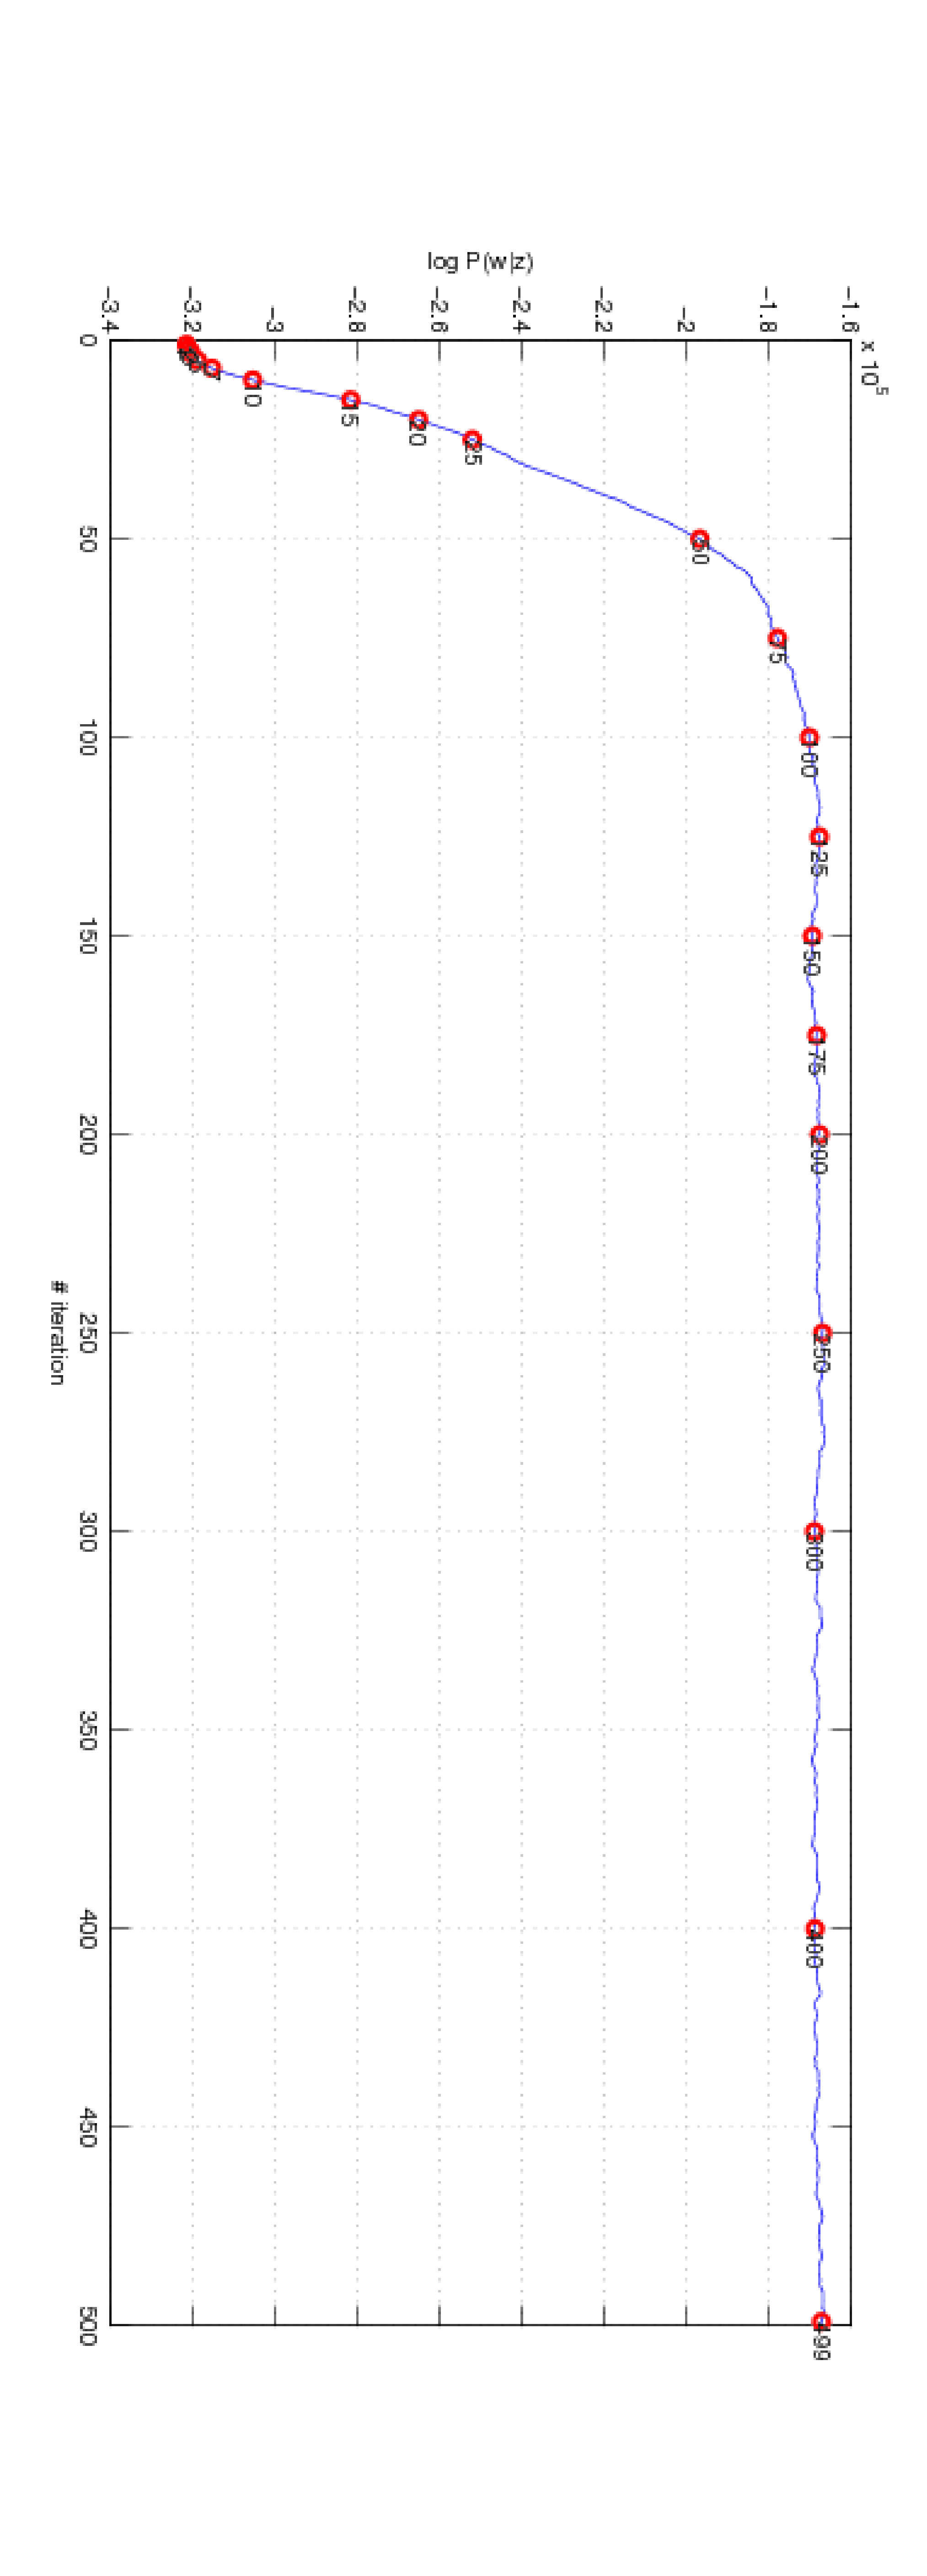
\includegraphics[width=0.5\columnwidth]{GriffithsExperiment_logPwz_rot}
  \hspace{-0.5cm}
  \includegraphics[width=0.6\columnwidth]{GriffithsExperiment_Images}
}
\caption{The result of running the Gibbs sampling algorithm to learn
  an LDA from synthetic data.  Each row of 10 images in the right pane
  visualizes the $\PWZ=\{\Pwz{k}\}_{k=1}^{K=10}$ estimated at
  those iterations indicated by red circles in the left pane.}
  \label{fig:correctness-test}
\end{figure}

The synthetic image data mentioned in \cite{lda_gibbs} is useful to
test the correctness of any implementation of LDA learning algorithm.
To synthesize this data set, we fix
$\PWZ=\{\Pwz{k}\}_{k=1}^{K=10}$ as visualized in
Fig.~\ref{fig:ground-truth-Phi} (also, Fig.~1 in \cite{lda_gibbs}),
set $\vtopicprior=[1]$, the number of words/pixels in each
document/image $d=100$.  Because every image has $5\times{}5$ pixels,
the vocabulary size is 25.\footnote{All these settings are identical
  with those described in \cite{lda_gibbs}.}

Fig.~\ref{fig:correctness-test} shows the result of running Gibbs
sampling to learn an LDA from this testing data set, where the left
pane shows the convergence of the likelihood, and the right pane shows
the updating process of $\PWZ$ along the iterations of the
algorithm.  The 20 rows of images in the right pane are visualizations
of $\PWZ$ estimated at the iterations of 1, 2, 3, 5, 7, , 10, 15,
20, 25, 50, 75, 100, 125, 150, 175, , 200, 250, 300, 400, 499.  From
this figure we can see that since iteration 100, the estimated
$\PWZ$ is almost identical to Fig.~1(a) of \cite{lda_gibbs}.



\section{Acknowledgement}

Thanks go to Gregor Heinrich and Xuerui Wang for their gentle
explanation of some math details.


%%% Local Variables:
%%% mode: latex
%%% TeX-master: "llt"
%%% End:
